\documentclass[hyperref={pdfpagelabels=false}]{beamer}
\usepackage{graphicx,lmodern,subfigure,ulem,color,graphicx,tikz,booktabs,natbib}
\usepackage{mathrsfs}
\usetheme{Warsaw}
%\definecolor{beamer@blendedblue}{rgb}{0.1,0.5,0.1}
%\definecolor{ForestGreen}{RGB}{60, 140, 60}
%\setbeamercolor{structure}{fg=beamer@blendedblue}
\setbeamertemplate{navigation symbols}{}
\setbeamertemplate{footline}[frame number]
\bibliographystyle{chicago}
\newcommand{\spitem}{\vspace{.3cm}\item}
\newcommand{\elas}{$E_{labor}$}
%\def \FigPath {Users\th3\Documents\Job_Market_Paper\Code\Figures} 


\title{Uncertainty Shocks}
\author{Marco Brianti}
\institute{Boston College}
\date{September 2018}


\begin{document}
	
	\frame{\titlepage \begin{center} Dissertation Workshop \end{center} }
	
	
		\frame{\frametitle{Two Possible Avenues}
		
		
		\begin{enumerate}
			\item News-noise driven uncertainty
			
			\
			
			\item Financial Shocks vs Uncertainty Shocks
		\end{enumerate}
		
		
	}

\frame{\frametitle{Credit Conditions and Uncertainty (I)}


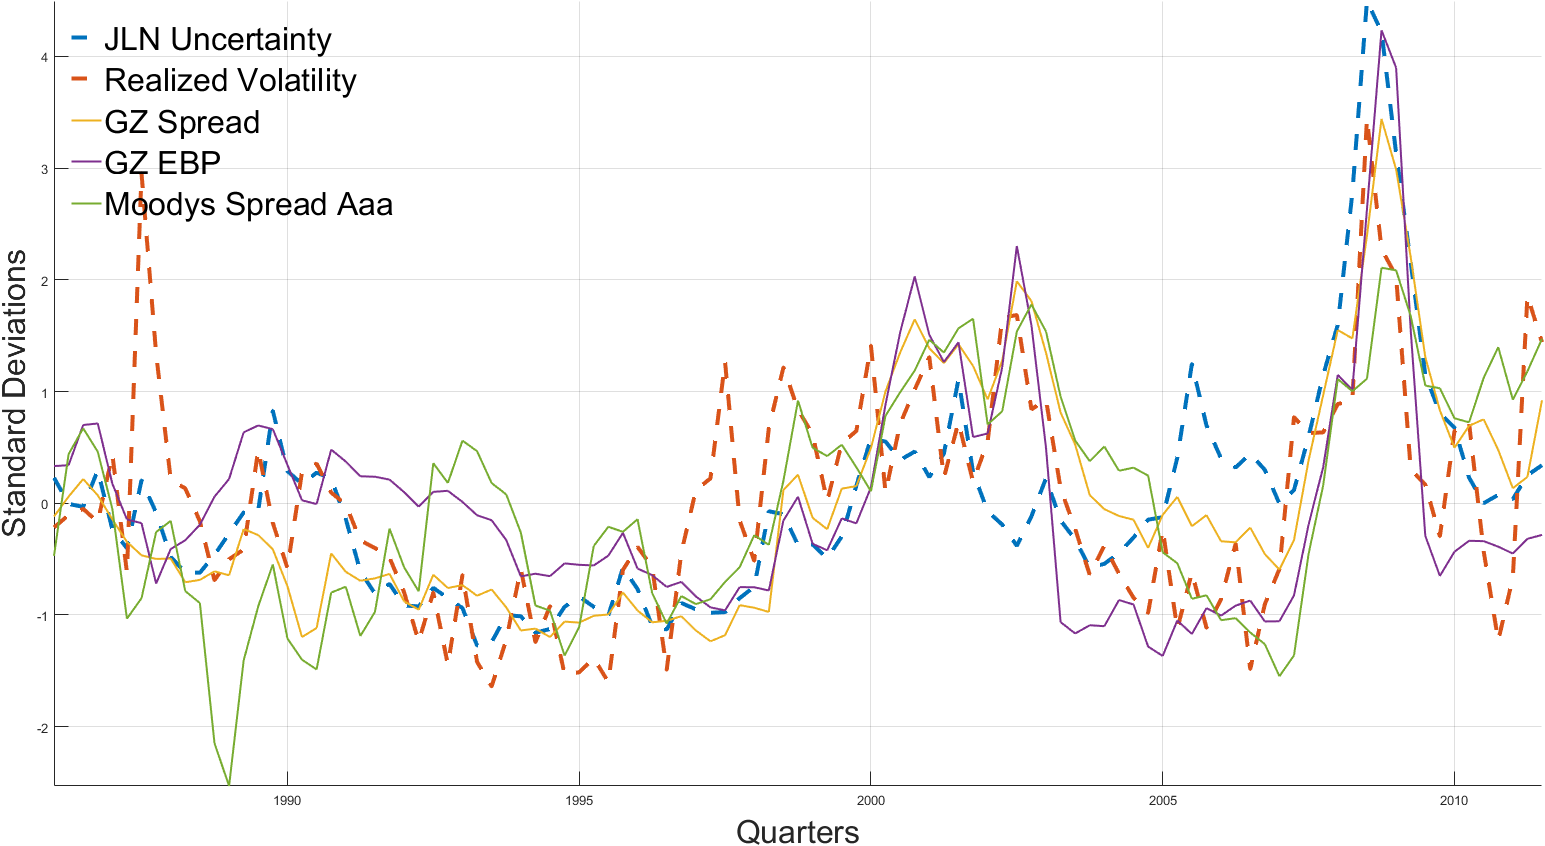
\includegraphics[scale=0.26]{Financial_Uncertainty}

\

Proxies for \textbf{credit conditions} and \textbf{uncertainty} are both countercyclical and tightly correlated.

}


\frame{\frametitle{Credit Conditions and Uncertainty (II)}
	
	
	\begin{table}
		\begin{tabular}{c||cccccc}
            & JLN         &      RV    & GZ  & EBP &    Moodys Aaa 	  \\
            \hline
            \hline
JLN	        &    1        &       -    &      -     &       -    &    -   \\
RV        	&    0.5865   &  1         &     -      &     -      &    -   \\ 
GZ       	&    0.7742   &  0.6247    &  1         &     -      &     -  \\
EBP      	&    0.6213   &  0.5621    &  0.7316    &  1         &     -  \\
Moodys Aaa	&    0.4386   &  0.4554    &  0.7993    &  0.5243    &    1   \\
	\end{tabular}
	\end{table}

\

\

As suggested by the graph above, all the variables are strongly correlated.

}


\frame{\frametitle{Financial Shocks and Uncertainty Shocks}
	
	Stock and Watson (2012); Caldara et al. (2016) among others shown that uncertainty shocks and financial shocks are deeply confounded.
	
	\
	
	\
	
	
	$$
	corr(\iota^{EBP}_t,\iota^{JLN}_t) \approx 0.45
	$$
	
	\
	
	\
	
	
	where $\iota^{EBP}_t$ is an unpredictable innovation in the \textbf{excess bond premium} from Gilchrist and Zakrajzek (2012) and $\iota^{JLN}_t$ is an unpredictable innovation in the \textbf{uncertainty proxy} from Jurado et al. (2015).
	

	

	
	
	
}

\frame{\frametitle{Both a theoretical and empirical question}

	Literature did not succeed yet to disentangle the two exogenous sources for two main reasons:
\begin{enumerate}
	\item Simultaneity
	\begin{itemize}
		\item Both types of variables are fast moving
				\end{itemize}	
			\item Observationally equivalence
			
			\begin{itemize}
			\item They have the same qualitative effects on prices and quantities
\end{itemize}
\end{enumerate}

\

\

As a result, both \textbf{zero-impact restrictions} cannot be used and \textbf{internal instruments} are not available.
	
}

\frame{\frametitle{My contribution}
	
	I want to take a step back and show evidence and theory that financial and uncertainty shocks
	
	
	\begin{itemize}
		
		\item are not qualitatively equivalent, and
	
		
		\item they can be successfully disentangled.
		
		\end{itemize}
	
	\	
	
	\
	
	
	In particular, I will show evidence that there exists a set of variables which respond differently to financial and uncertainty shocks. 
	\begin{itemize}
		\item there exists an \textbf{economic intuition} for this response
		\item those variables can be used as \textbf{internal instruments}
	\end{itemize}
}
	
		\frame{\frametitle{Variables of Interest by Bureau of Economic Analysis}
		

\textbf{Cash Flow} is defined as (i) undistributed corporate profits plus (ii) consumption of fixed capital minus (iii) net capital transfers paid.

\

where 

\begin{enumerate}
	\item \textbf{Undistributed corporate profits} are defined as (i) corporate profits minus (ii) dividends
	\item \textbf{consumption of fixed capital} can be simply interpreted as capital depreciation
	\item \textbf{net capital transfers paid} are unrequited transfers associated with the acquisition or disposal of assets.
\end{enumerate}

\

\textbf{Cash Flow} is a profit-related measure of \textbf{internal funds} available for investment. [The NIPA Handbook, December 2015]

	}


\frame{\frametitle{Partial Equilibrium Analysis (I)}
	
	Decrease in the risk bearing capacity of the financial sector. 
	
	\begin{figure}[plain]
		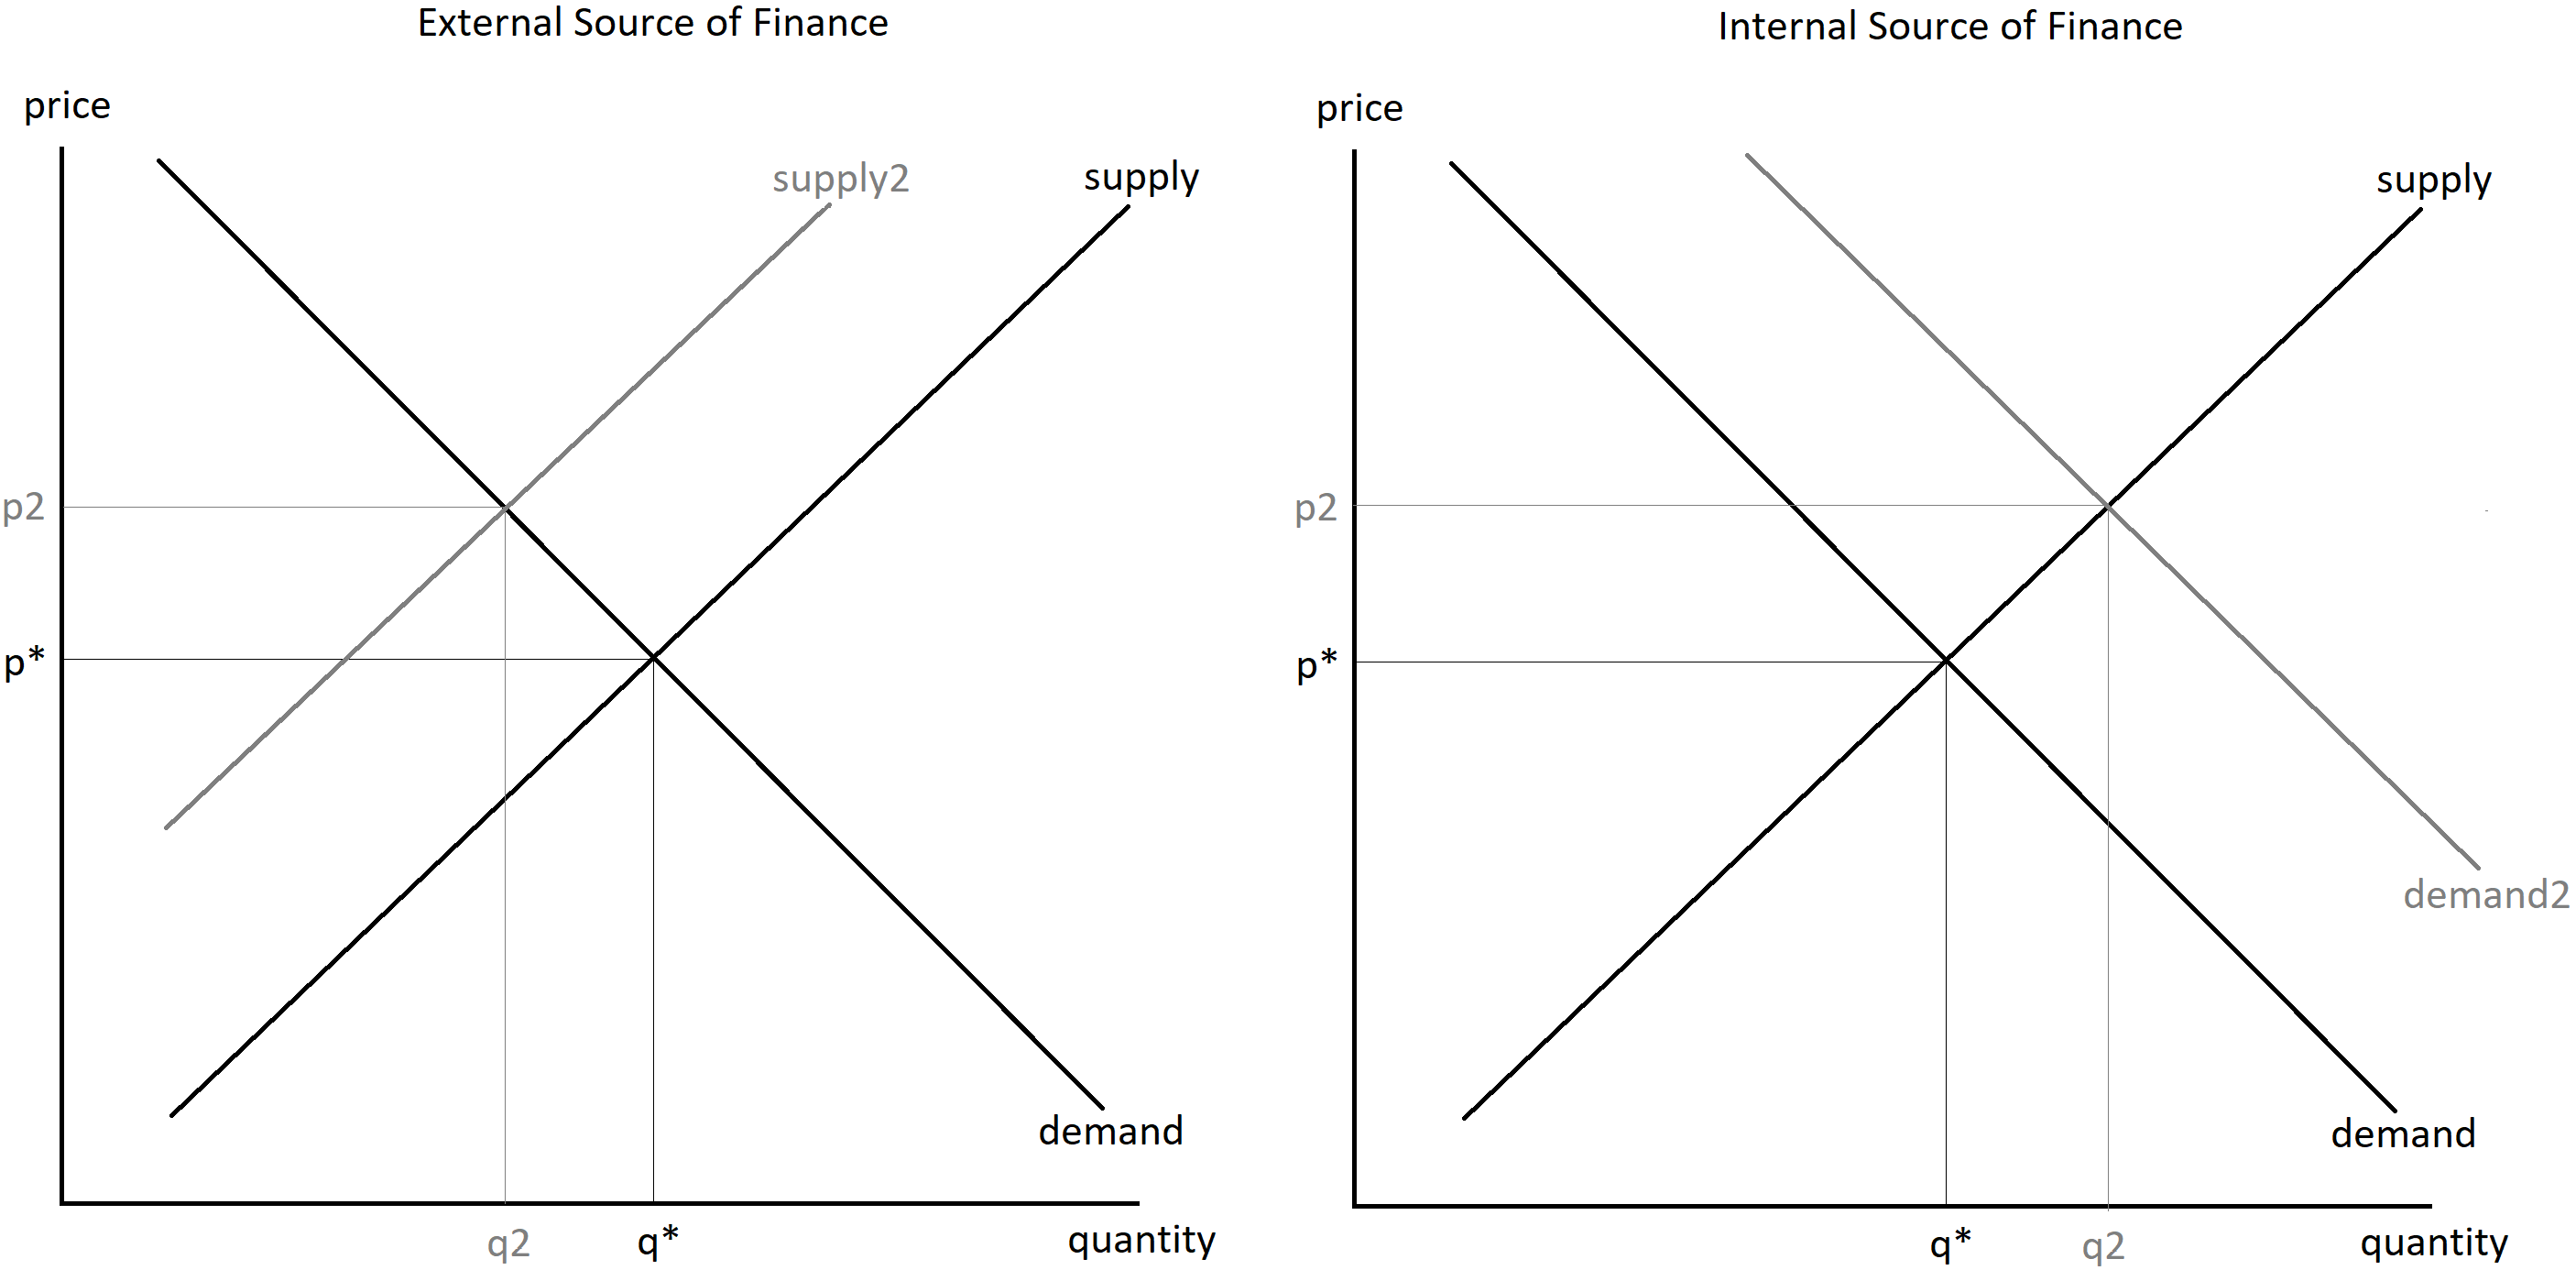
\includegraphics[scale=0.13]{fig_financial_supply_demand_F}
	\end{figure}
	
	Notice that I am taking as given the supply of internal source of finance. 
}

\frame{\frametitle{Partial Equilibrium Analysis (II)}
	
	Increase in the level of uncertainty. 
	
	\begin{figure}[plain]
		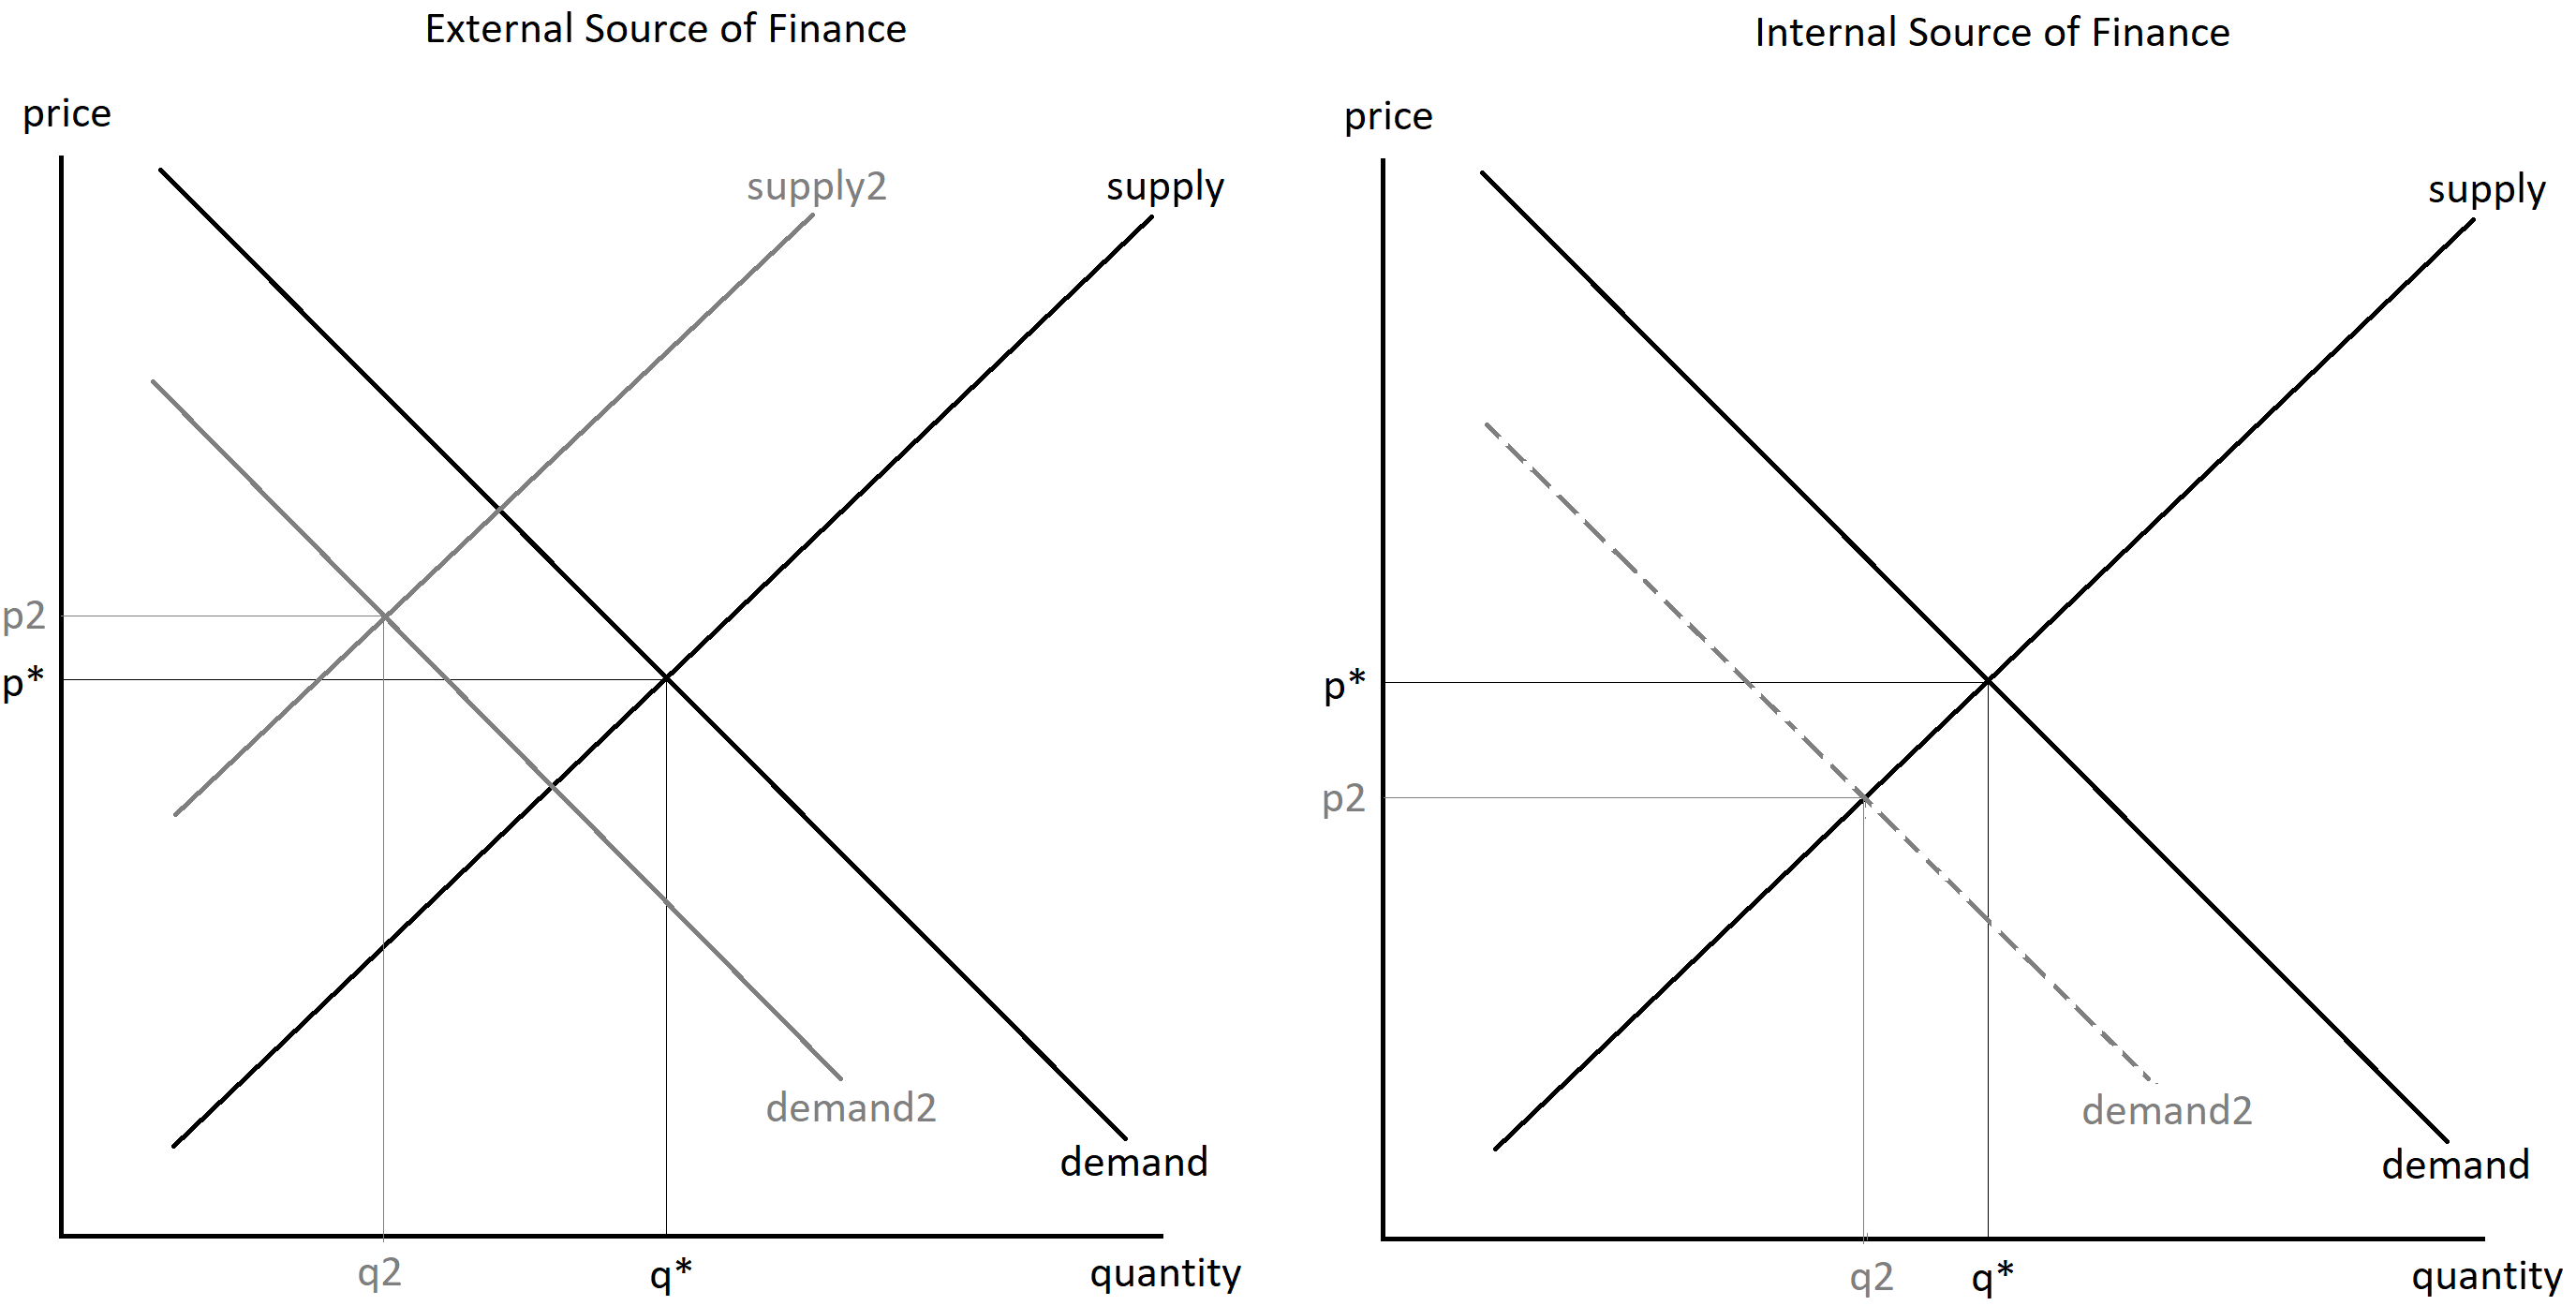
\includegraphics[scale=0.13]{fig_financial_supply_demand_U}
	\end{figure}
	
	Notice that I am taking as given the supply of internal source of finance. 
	
}


\frame{\frametitle{Economic Intuition}
	
	
	\begin{itemize}
		
		\item 	After a \textbf{decrease in credit supply}, quantity of the internal source of finance should increase.
		
		\begin{itemize}
			\item Controlling for supply of internal funds cash flow should increase.
		\end{itemize}
		
		\
		
		\
		
		\item After an \textbf{increase in uncertainty}, quantity of the internal source of finance should either decrease or remain unchanged.
		
	\begin{itemize}
	\item Controlling for supply of internal funds cash flow should either decrease or remain unchanged.
\end{itemize}
		
		
		
		
	\end{itemize}
	
}	
	
	\frame{\frametitle{Controlling for the Supply of Internal Funds}	
		
		The main source of internal funds available for investment is the \textbf{flow profit} of the current year.
		
		\
		
		In order to control for general equilibrium effect, cash flow needs to be normalized by the corporate profit.
		
		In particular, normalized cash flow can be thought as an index between $0$ and $1$
		\begin{itemize}
			\item If the index is equal to zero, current profits are fully distributed outside the firm
			\item If index is equal to one, current profits are going to be internally used
		\end{itemize}
	
	
	
	
	

		
	}
	

\frame{\frametitle{Suggestive Evidence}
	
	Run the following regression,
	
	\
	
	$$
	\tilde{CF}_t = \alpha + B(L)X_{t-1} + \beta^{F} \iota_t^F + \beta^{U} \iota_t^U + \varepsilon_t
	$$
	
	\
	
	where 
	
	\
	
	\begin{itemize}
		
		
		\item $\tilde{CF}_t$ is cash flow normalized by corporate profits
		
		\
		
		\item $X_{t-1}$ is a set of variables to control for predictable part of $\tilde{CF}_t$
		
		\
		
		\item $\iota_t^F$ and $\iota_t^U$ are the unpredictable part of financial conditions and uncertainty, respectively
		
		
	\end{itemize}


	
}

	
	\frame{\frametitle{Results}
		

Benchmark regression,
$$
\tilde{CF}_t = \alpha + B(L)X_{t-1} + \beta^{F} F_t + \beta^{U} U_t + \varepsilon_t
$$

\

\

\begin{itemize}
	\item $\beta^F$ is always positive and significant at $1$\%.
	
	\
	
	\
	
	\item $\beta^U$ is either negative or not significant. 
\end{itemize}
		
	}




\end{document}